\documentclass{article}
\usepackage{graphicx}
\usepackage{hyperref}
\usepackage{caption}
\usepackage{subcaption}
\usepackage[dutch]{babel}

\begin{document}

\begin{center}
	\huge{Wiskunde in Kunst}\\
	\LARGE{Opdracht 1} \\
	
	\vspace{2cm}
	
	\Large{Circle Limit III}\\
	\large{\textit{M. C. Escher}}
	
	\begin{figure}[htp]
		\centering
		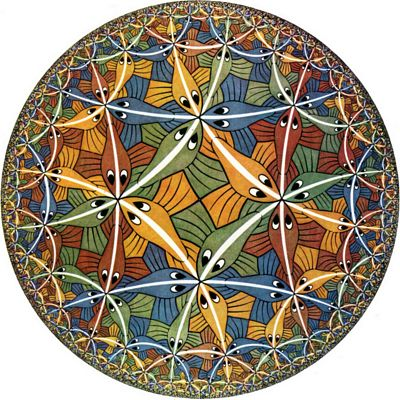
\includegraphics[scale=1.00]{Escher_Circle_Limit_III.jpg}
		\label{}
	\end{figure}
	
	\vfill
	\Large{Marcelo Dias Avelino} \hfill \large{0840416}
\end{center}

\pagebreak

\tableofcontents

\pagebreak

\section{Kunstwerk}

De kunstwerk \textit{Circle Limit III} is een houtsnede stuk gemaakt door de nederlandse kunstenaar Maurits Cornelis Escher (meestal gerefereerd als M. C. Escher). Escher heeft dit kunstwerk gemaakt in 1959 in zijn huis in Baarn, Utrecht. Hij verhuisde hierheen in 1941 vanuit Brussel vanwege de tweede wereld oorlog.

\end{document}
